\documentclass[12pt]{article}
\usepackage{graphicx}
\usepackage{subfigure}
\usepackage{amsmath}
\usepackage{geometry}
\geometry{legalpaper, portrait, margin=1in}
\usepackage{mhchem}
\usepackage[affil-it]{authblk}

\begin{document}
\title{refnx - Neutron and X-ray reflectometry analysis in Python}
\author[1,*]{Andrew Nelson}
\author[2]{Stuart Prescott}

\affil[1]{% 
 Australian Nuclear Science and Technology Organisation, Locked Bag 2001, Kirrawee DC, NSW 2232, Australia}
\affil[2]{School of Chemical Engineering, University of New South Wales,  Sydney, NSW, Australia}
\affil[*]{Corresponding author: Andrew.Nelson@ansto.gov.au}

\date{\today}

\newcommand{\refnx}{\emph{refnx }}
\newcommand{\Objective}{\textbf{Objective }}
\newcommand{\Parameter}{\textbf{Parameter }}
\newcommand{\Structure}{\textbf{Structure }}
\newcommand{\Slab}{\textbf{Slab }}
\newcommand{\Component}{\textbf{Component }}
\newcommand{\LipidLeaflet}{\textbf{LipidLeaflet }}
\newcommand{\Spline}{\textbf{Spline }}
\newcommand{\conda}{\emph{conda }}
\newcommand{\MixedReflectModel}{\emph{MixedReflectModel }}
\newcommand{\pip}{\emph{pip }}
\newcommand{\NumPy}{\emph{NumPy }}
\newcommand{\Cython}{\emph{Cython }}
\newcommand{\Jupyter}{\emph{Jupyter }}
\newcommand{\ipywidgets}{\emph{ipywidgets }}

\maketitle

\begin{abstract}
The \refnx package is designed for object-oriented model-based analysis of neutron and X-ray reflectometry data in Python. It is cross platform, and has been tested on Linux, macOS, and Windows.
Structure construction is modular, being composed from a series of Components that each describe a subset of the interface. These Components (such as LipidLeaflet, or Spline) allow the user to parameterise their model in terms of physically relevant parameters. The Model and data are used to create an Objective, which is used to calculate residuals, log-likelihood, and log-prior probabilities of the system. Objectives are combined to perform co-refinement of multiple datasets, and mixed-area models. All parameters in the system can have a variety of Bounds applied; these bounds consist of probability distributions which represent their prior probability. The prior probability encodes a user's knowledge about the Parameter values, which allows the curve-fitting engine to direct solutions toward a more probable parameter space. Extra prior probability terms can be defined for Components, over and above those available from the Parameters alone.
Algebraic Parameter constraints are available.
The powerful curve-fitting engine offers the choice of using a normal least-squares fitting approach (with a variety of global and gradient-based optimizers) or a Bayesian approach using Markov Chain Monte Carlo to investigate the posterior distribution of the model parameters. The Bayesian approach is useful in examining parameter covariances, model selection, and variability in the resulting scattering length density profiles.

The whole package is designed with a focus on reproducible research; its use in \Jupyter notebooks (which includes a graphical user interface), and subsequent distribution of those notebooks as supplementary information, permits scientists to straightforwardly reproduce analyses made by others.
\end{abstract}

\subsection*{Introduction}
The use of specular X-ray and neutron reflectometry for morphological characterisation of thin films on the approximate size range [10, 5000]$\AA$ has exploded over the past years \cite{Wood2017, Daillant2009}. Most neutron and X-ray sources have instruments to perform reflectometry measurements, and there is an ongoing need for accessible software programs for users of those instruments to analyse their data in a straightforward fashion, including the co-refinement of multiple contrast datasets.  Several programs are available for this purpose, with a variety of different features \cite{Bjorck2007, Gerelli2016, Kienzle2011, Nelson2006}. These programs typically create a model of the interface, and incrementally refine the model against the data using least-squares, or use Bayesian approaches \cite{Sivia2006, 2010arXiv1008.4686H} to examine the posterior probability distribution of the parameters (i.e. the statistical variation of the parameters in a model).

Given that there are more and more publications arising from the reflectometry technique, it is vital that the analysis is reproducible. Reproducibility in research is an underlying principle of science. Unfortunately, it is not always possible to reproduce the results of others \cite{Stark2018}, because there is frequently not enough information provided in journal articles to repeat the analyses. Even if the datasets and software packages used to analyse them are supplied in supplementary information (most often they are not), a comprehensive set of instructions would need to be provided.
One example for addressing this reproducibility issue are the guidelines in the small-angle scattering community for the deposition of data and and associated models \cite{Trewhella:jc5010}.

Here we outline a new reflectometry analysis package, \refnx (version number x.x is used in this paper \cite{refnx}), that can address the reproducibility issue for the reflectometry community as it is specifically designed for use in \Jupyter notebooks \cite{Kluyver:2016aa} using a Python kernel \footnote{We do not mean that other programs are irreproducible, rather that the information provided by scientists in journal articles is often lacking.}.
These notebooks are a mix of executable code cells and markup. An analysis performed in such a notebook can be appended as supplementary information, along with the data, to an article. Readers can then replicate the exact data analysis, provided they have set up the same computing environment. Setting up the computing environment is simplified using the \conda package manager \cite{conda}, and an environment file (although other approaches are available). To that end the \Jupyter notebooks for the example analysis performed in this paper are appended as supplementary information.

\refnx has a wide range of sophisticated modelling capabilities including: parameter constraints, description of prior probabilities on parameters using arbitrary probability distribution functions, modular construction of models using a variety of components that are user extensible, co-refinement of datasets, handling of patchy layers, a graphical user interface, resolution handling, Markov Chain Monte Carlo sampling of the posterior probability distributions, model selection, etc.

The posterior probability distribution in Bayesian statistics, Equation~\ref{eqn:1}, says the posterior probability distribution for the parameters is proportional to the product of the prior probability and the likelihood (or the sum of the log-probabilities).

\begin{gather} 
\label{eqn:1}\ p(\theta | D, I) \propto p(\theta | I)\times p(D | \theta, I)\\
p(D | \theta, I) = -\frac{1}{2} \sum [(\frac{y_n - model} {\sigma_n})^2 + log(\sigma_n^2)]\label{eqn:2}
\end{gather}

The posterior distribution, $p(\theta | I, D)$, is the probability of the parameters given the data, $D$, and prior knowledge about the system, $I$. 
The prior probability distribution, $p(\theta | I)$, is the state of knowledge that already exists about the parameters of interest, such as that obtained from other experiments.
The likelihood (Equation~\ref{eqn:2}), $p(D | \theta, I)$, is the probability of the observed data, $y_n$ (with uncertainties $\sigma_n$), given the model parameters and other prior information.  The posterior probability is sampled by encoding the likelihood and prior distributions and using Markov Chain Monte Carlo (MCMC) techniques \cite{emcee}.

\subsection*{Method}
\refnx is written in Python with an object-oriented design, Figure~\ref{fig:components}. As with \emph{Motofit} \cite{Nelson2006} it calculates reflectivity using the Abeles method \cite{Heavens1955} for specular reflection from a stratified medium.
The building block of the analysis is the \Parameter object which represents a model value, whether it is allowed to vary in a fit, and a bounds attribute. The bounds are a probability distribution - the simplest bound being a uniform distribution which would set lower and upper limits for the parameter. This probability distribution is the prior probability for the parameter. Any of the \emph{scipy.stats} \cite{Jones2001-2017} continuous distributions, or distributions created by the user, can be used for this purpose. Algebraic relationships between \Parameter can be applied using constraints.
The \Structure object represents the interfacial model, comprising of individual \Component objects in series. Each \Component represents a subset of the interface and contains several physically relevant Parameters. The simplest \Component is a \Slab, which has a uniform scattering length density (SLD), thickness, roughness, and volume fraction of solvent. The simplest models are simply a series of \Slab. More sophisticated components include \LipidLeaflet and \Spline. \Spline is designed for freeform modelling of an SLD profile using spline interpolation. In addition to its constituent parameters each \Component can also contribute to the log-prior probability. This is useful when a \Component has a derived value, such as surface coverage, which is already known, and can be included as prior knowledge of the system. Each \Component has a \emph{slabs} property that represents the strata for its particular subset of the interface. A \Slab object has a single slice because it is a single thickness of uniform SLD. A \LipidLeaflet can be made of two slices (head/tail regions), but the \Spline Component has many. These slices have uniform SLD, and use the Nevot-Croce \cite{Nevot1980} to describe roughness between them. If a different roughness model is required then a 'microsliced' \Component could be written to accomodate that.
The \Structure object is used to construct a \textbf{ReflectModel} object. This object is responsible for calculating the resolution smeared reflectivity of the \Structure, scaling the data, and adding a linear background (via the scale and background Parameters). There are different types of smearing available - constant dQ/Q, point by point resolution smearing from the dataset of interest, or via a smearing kernel of arbitrary shape \cite{Nelson2014}.
The \Objective class uses the \textbf{ReflectModel} and a dataset \textbf{Data1D} to calculate $\chi^2$, log-likelihood, log-prior, residuals, and the generative model. The \Objective can be given a \textbf{Transform} object to permit fitting as log-R vs Q, $RQ^4$ vs Q, or lin-R vs Q. Several \Objective can be combined to form a \textbf{GlobalObjective} for co-refinement. The object-oriented nature allows \Parameter, \Component to be reused throughout the setup, thereby facilitating co-refinement. For an example please see \textbf{lipid.ipynb} in the supporting information.
The \Objective statistics are used directly by the \textbf{CurveFitter} class to perform least-square fitting or Bayesian MCMC of the system. \refnx uses the \emph{scipy} package for least-squares analysis (DifferentialEvolution, Levenberg Marquardt, LBFGSB - Limited Broyden–Fletcher–Goldfarb–Shanno with bounds) and the  \emph{emcee} package \cite{emcee} for affine invariant MCMC ensemble sampling of the posterior distribution of the parameters. The likelihoods used in MCMC and least-squares assume that the measurement errors are normally distributed, Equation~\ref{eqn:2}. However, other types of measurement errors (e.g. Poissonian) could be implemented by a subclass of \Objective and overriding the log-likelihood method.
Parallelisation of the sampling is done automatically, and can use MPI on a cluster for greater parallelisation. Visualisation of the samples produced by MCMC sampling is done using the \emph{corner} package \cite{corner} for scatter plot matrices. On the conclusion of a fit/sampling run each \Parameter is updated and given a standard error. For the sampling these represent the median and half the [15.87, 84.13] percentile range respectively; the latter approximates the standard deviation for a normally distributed statistic.

\begin{figure}
  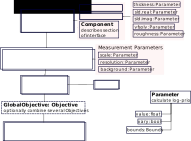
\includegraphics[width=\linewidth]{components}
  \caption{Schematic showing the relationship between classes that make up a typical reflectometry curve-fitting problem.}
  \label{fig:components}
\end{figure}

To make it easy to create quick models, and to ease the learning curve, an ipywidgets \cite{ipywidgets} based fitting GUI can be created in a \Jupyter notebook, Figure~\ref{fig:gui}. This GUI builds slab based models for analysing a single dataset, but can be used as a stepping point for building more advanced models via the 'To code' code generation button.

\begin{figure}
  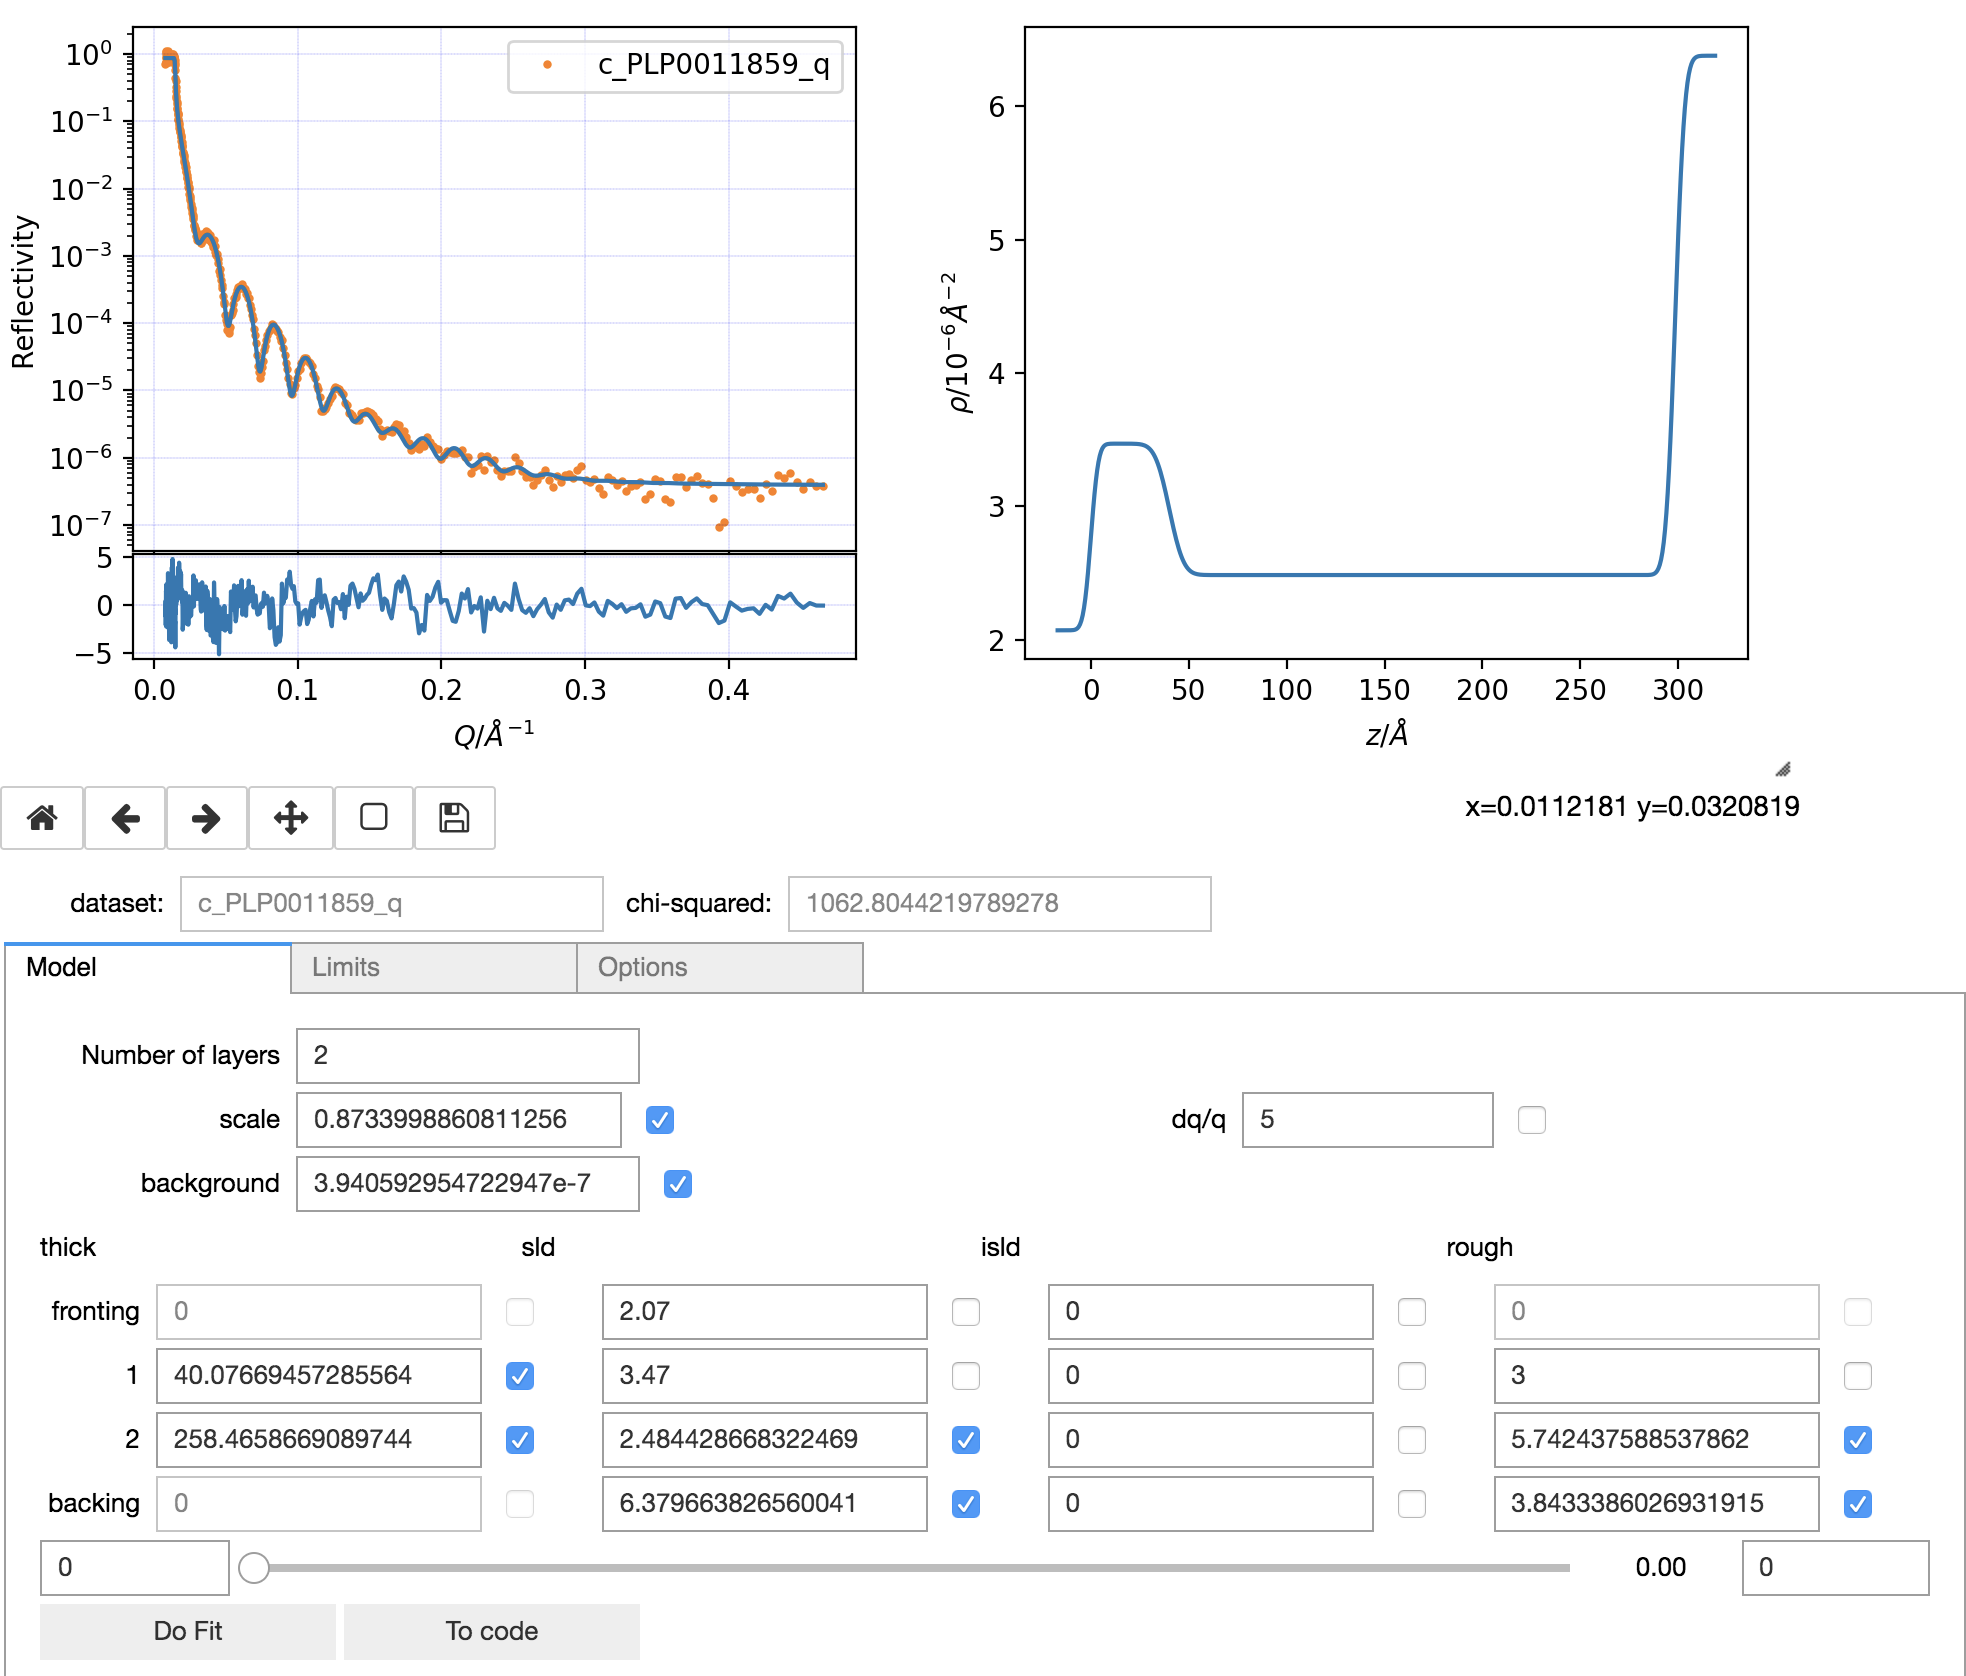
\includegraphics[width=\linewidth]{./datasets/gui.png}
  \caption{Screenshot of the \Jupyter/\ipywidgets GUI. \Jupyter notebook available in supporting information.}
  \label{fig:gui}
\end{figure}

\subsection*{Example}
Neutron reflectometry is an ideal technique for the study of biologically relevant lipid membrane mimics and their interactions with proteins, etc. Multiple contrast variation measurements are necessary to reduce modelling ambiguity (due to loss of phase information in the scattering experiment) and improve the ability to determine the structure of various components in the system. The gold standard approach for analysis of these datasets is co-refinement with a common model, and to parameterise the model in terms of chemically relevant parameters, such as area per molecule. Sometimes a patchy coverage (distinct to low area per molecule) necessitates the use of an (incoherent) sum of reflectivities from different areas. \refnx has functionality for all these requirements, such as the \LipidLeaflet component for describing the head and tail groups of a lipid leaflet, and \MixedReflectModel. It is straightforward to develop/modify new components for different structural functionality, a consequence of the object-oriented approach. Here the \LipidLeaflet is used to co-refine three contrasts (\ce{D_2O}, \ce{Si} contrast match [hdmix, SLD=$2.07\times10^{-6}\AA^{-2}$], and \ce{H_2O}) of a 1,2-dimyristoyl-sn-glycero-3-phosphocholine (DMPC) bilayer at the solid-liquid interface, Figure \ref{fig:global_fit} \footnote{The validity of \LipidLeaflet does depend on the area per molecule being equal for the headgroup and tailgroup regions, as pointed out by Gerelli \cite{Gerelli2016}, which can be violated if there are guest molecules that insert in the membrane.}. The corner plot (Figure \ref{fig:corner}) produced from the MCMC analysis shows the covariance between parameters, with an area per molecule of 57$\AA\pm1$. Figures~\ref{fig:global_fit} and \ref{fig:d2o_sld_spread} show the probability distribution of the generative model around the data and in the SLD profile. These are obtained by random samples from the MCMC chain. The spread in SLD profiles is used to determine what range of structures is consistent with the data. Multi-modalities in these SLD profiles can be due to statistical uncertainties, the Q ranges measured, and the loss of phase information in NR \cite{Majkrzak1999, Heinrich2009}.
%TODO use exact area per molecule, and use a reference for the Xray analysis

\begin{figure}%
\centering
\subfigure{%
\label{fig:global_fit}%
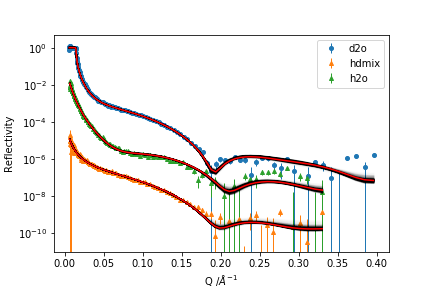
\includegraphics[width=5in]{./datasets/global_fit.png}}\hspace{1em}%
\subfigure{%
\label{fig:d2o_sld_spread}%
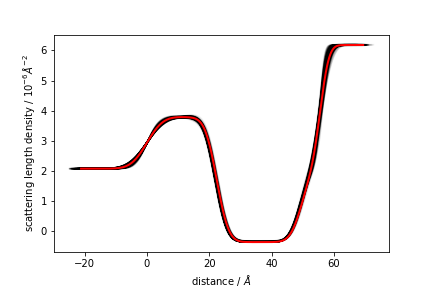
\includegraphics[width=5in]{./datasets/d2o_sld_spread.png}}\\%
\caption{a) Reflectivity from a DMPC bilayer measured at three contrasts, with median in red, and 500 samples from the posterior distribution. Dataset for \ce{Si} match offset by 0.1, \ce{H_2O} contrast offset by 0.001. b) SLD profile of the \ce{D_2O} model showing 500 samples from the posterior distribution, as well as the median. \Jupyter notebook used for the analysis is attached in the supporting information.}
\end{figure}

\begin{figure}
  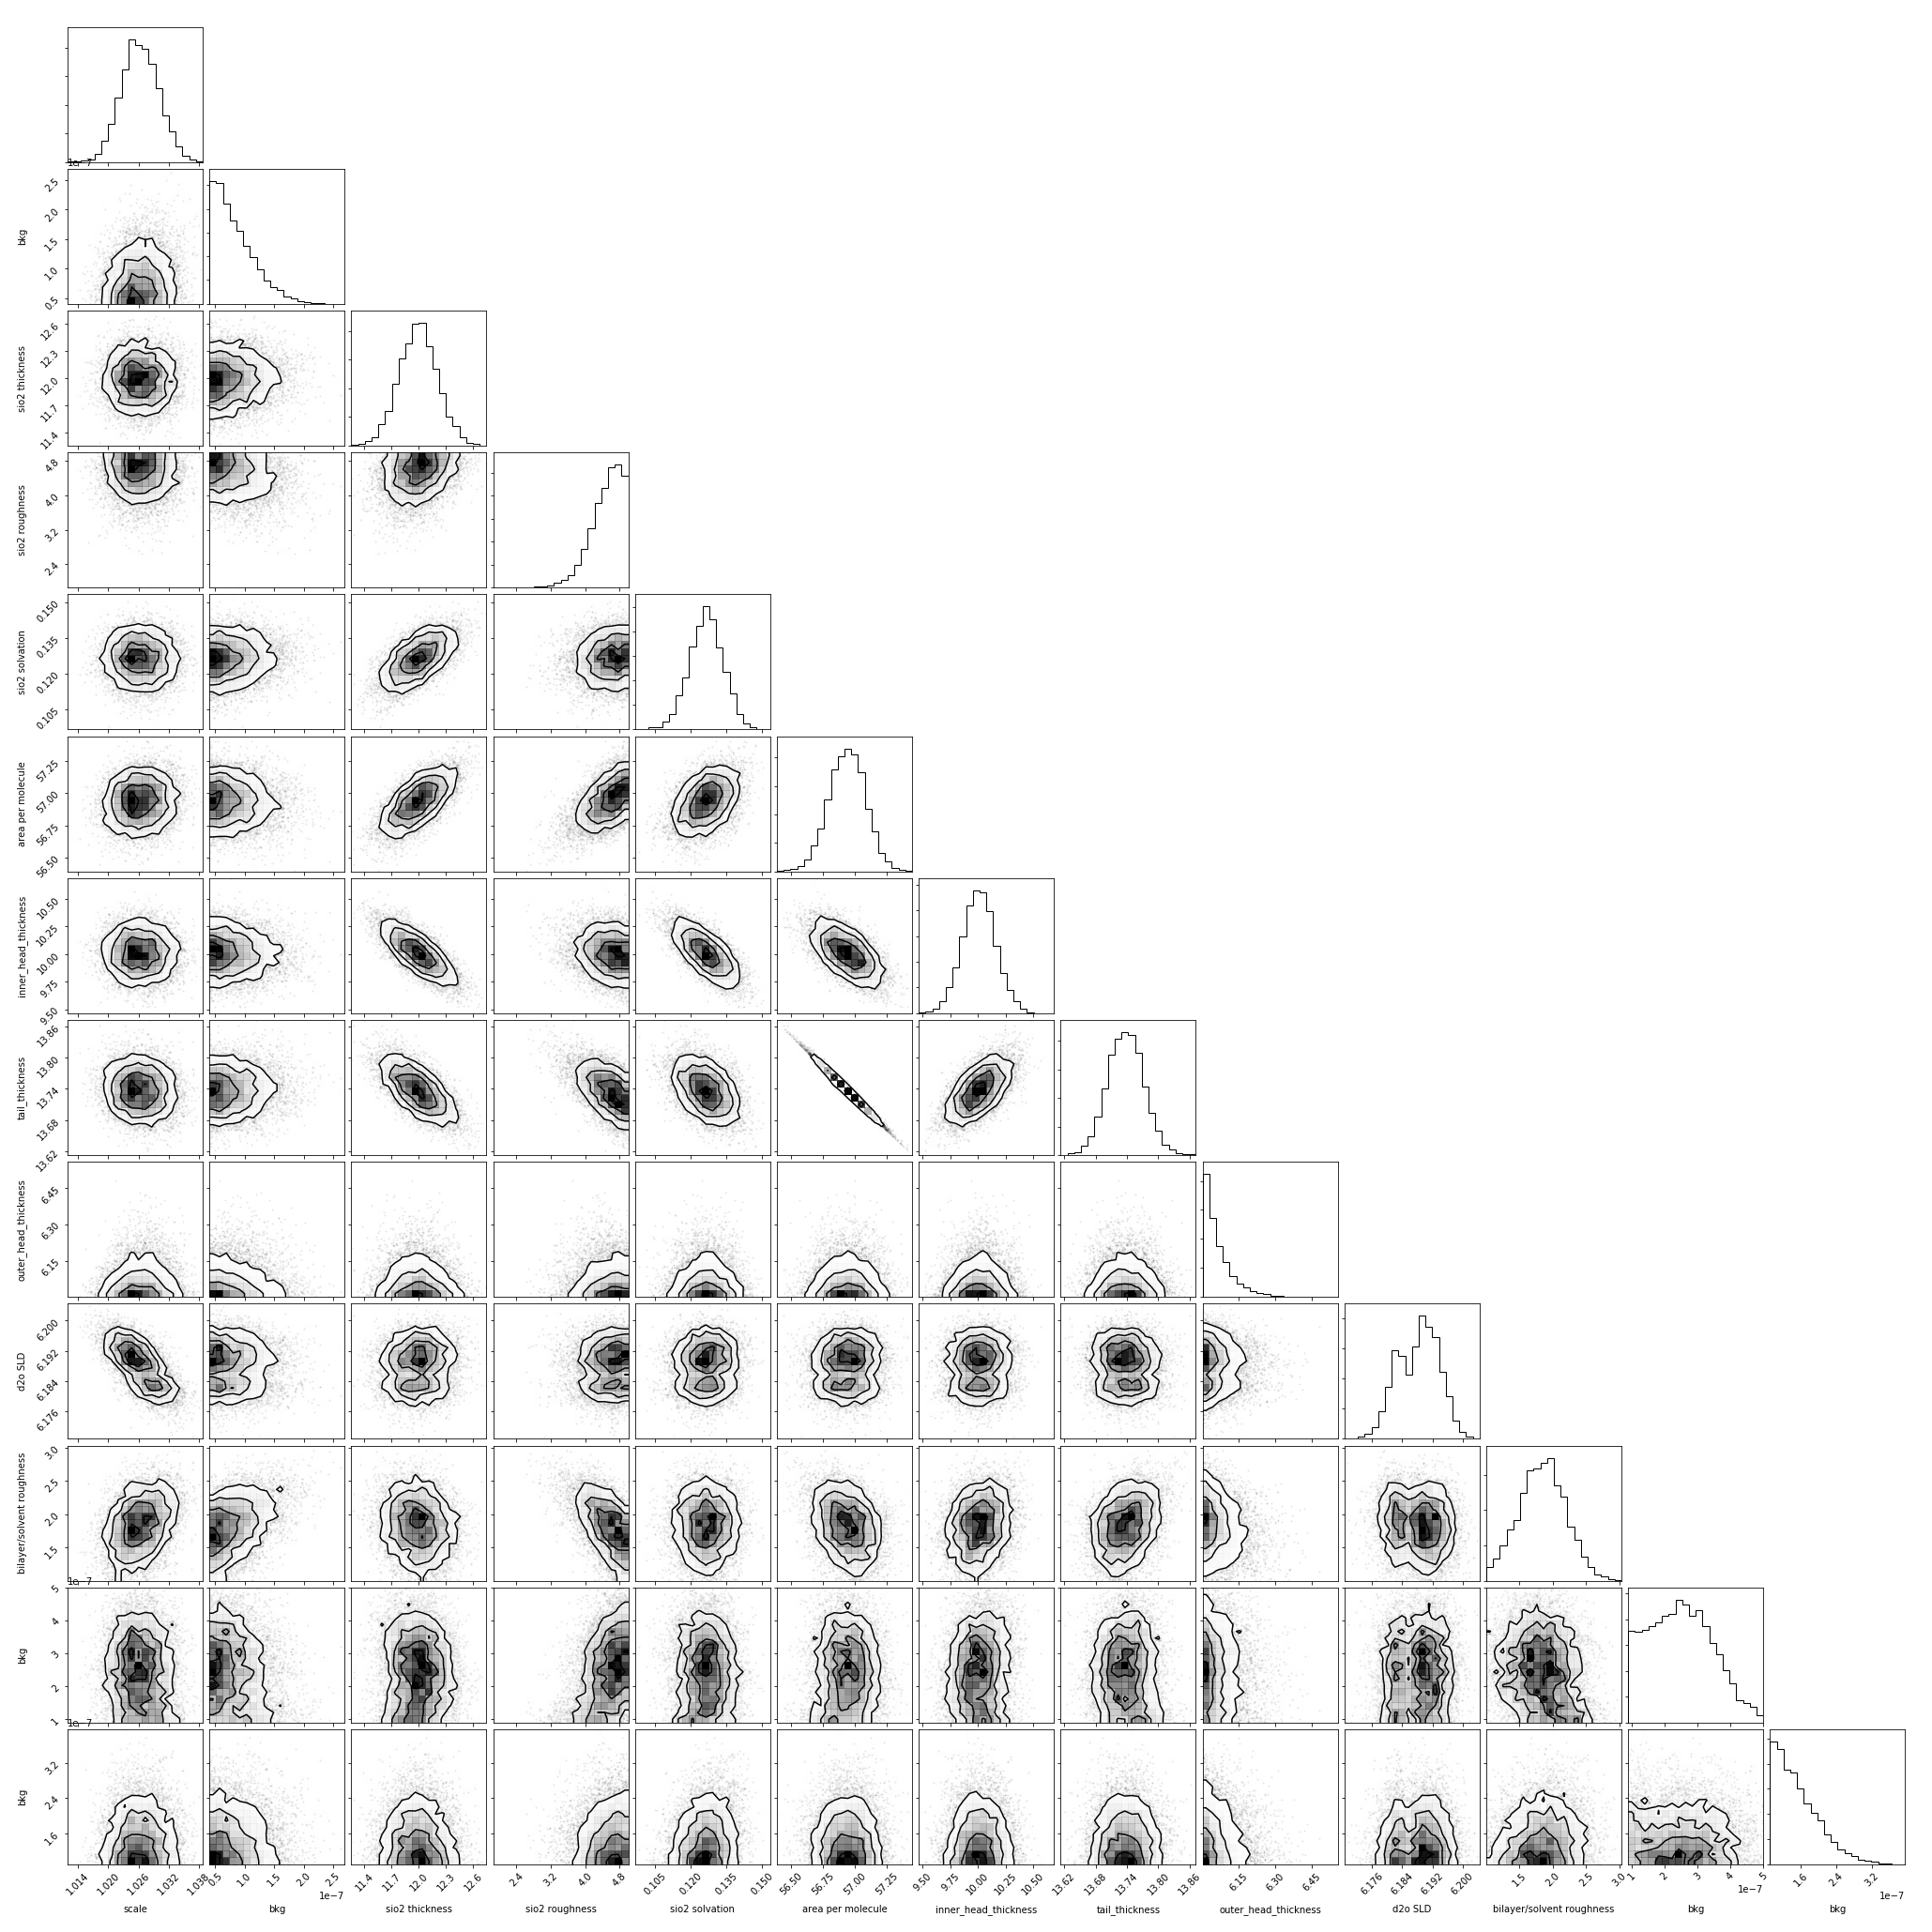
\includegraphics[width=\linewidth]{./datasets/corner}
  \caption{Corner plot for the varying parameters of DMPC bilayers measured at three contrasts.}
  \label{fig:corner}
\end{figure}

 
\subsection*{Distribution and Modification}
Each submodule in \refnx possesses its own unit testing code for checking that the functions and classes in the module operate correctly, both individually and collectively. For example, there are tests that check that the reflectivity of a model is calculated correctly, or that the behaviour of a function is correct for the different possible inputs and code paths through it. Since the test suite is an integral part of the package each installation is testable.
 
 The source code for \refnx is held in a version controlled git repository hosted on github at https://www.github.com/refnx/refnx. Contributors create their own fork of the main \refnx repository, and create a feature branch to which they make modifications. They then submit a pull request (PR) against the main repository. The modifications made in the PR are checked on continuous integration (CI) web-services which run the test suite against a matrix of Python versions on the macOS, Linux and Windows operating systems. If the tests pass, and the changes are considered useful, then the features are merged into the main repository. When a sufficient number of features have accumulated a new release is made. Successive releases have an incrementing semantic version number which can be obtained from the installed package, with each release being given its own DOI.

 The recommended way of using \refnx is from a \conda environment (a package, dependency and environment manager for software), using the pre-compiled distributables on the \refnx conda-forge channel. These distributables are made as part of the release process using the same CI web-services used to test the code. The matrix of distributables cover the major Python versions currently in use, across the macOS/Windows/Linux operating systems. Alternatively the package can be installed from source, either directly from the git repository, or via pip from the version uploaded to PyPI (https://pypi.python.org/pypi/refnx). Building from source requires a C compiler and the \Cython and \NumPy packages to be installed. It's important to note that for reproducible research purposes both \conda and \pip can be used to install a specific version of \refnx.
 
\refnx is released under the BSD permissive open source licence. In addition its dependencies are released under open source licences which mean that use is free of cost to the end user.

\subsection*{Conclusions}\label{conclusions}
\refnx is a powerful tool for least-squares or Bayesian analysis of neutron and X-ray reflectometry data that is ideally usable for reproducible research with \Jupyter notebooks. Its features include: MCMC sampling of posterior distribution for parameters, structural models constructed from modular components with physically relevant parameterisation, interparameter constraints, mixed area models, co-refinement of multiple datasets, probability distributions for parameter bounds used directly for log-prior terms, and a \Jupyter/\ipywidgets GUI

\subsection*{Acknowledgements}
We acknowledge Anton Le Brun for the provision of the lipid bilayer datasets in the example.
%TODO insert name

\subsection*{Supporting information}
\textbf{gui.ipynb} - \Jupyter notebook used to create the GUI screenshot.\\
\textbf{lipid.ipynb} - \Jupyter notebook used for the lipid analysis example

\bibliography{main}{}
\bibliographystyle{unsrt}
\end{document}